\documentclass[a4paper,titlepage,openright,12pt]{report}

\usepackage{graphicx}
%\usepackage{epsfig}

\usepackage[font=footnotesize]{subfig}
\usepackage{float}
\usepackage{fancyhdr}
\usepackage{makeidx}
\usepackage[nottoc,notlot,notlof]{tocbibind}
\usepackage{supertabular}
\usepackage{array}
\usepackage{setspace}
\usepackage{enumerate}
\usepackage{rotating}
\usepackage{moreverb}
\usepackage{multirow}
\usepackage{amsmath}
\usepackage{amsthm}
\usepackage{amssymb}
\usepackage{captcont}
\usepackage{verbatim}
\usepackage{titlesec}
\usepackage{url}
\usepackage{hyperref}
\usepackage{lipsum}
\usepackage{changepage}

%%%%%%%%%%%%%%%%%%%%%%%%%%%%%%%%%%%%%%%%%%%%%%%%%%%%%%%%%%%%

%\usepackage[algoruled]{algorithm2e}
%\usepackage[figure,algoruled]{algorithm2e}
%\usepackage[figure,boxruled]{algorithm2e}

%\newtheorem{theorem}{Theorem}
%\newtheorem{corollary}[theorem]{Corollary}
%\newtheorem{conjecture}[theorem]{Conjecture}
%\newtheorem{lemma}[theorem]{Lemma}
%\newtheorem{proposition}[theorem]{Proposition}
%\newtheorem{definition}[theorem]{Definition}
%\newtheorem{Example}[theorem]{Example}
%\newtheorem{axiom}{Axiom}
%\newtheorem{remark}{Remark}
%\newtheorem{exercise}{Exercise}[section]
%\newtheorem{fact}[theorem]{Fact}
%\newtheorem{property}[theorem]{Property}

%%%%%%%%%%%%%%%%%%%%%%%%%%%%%%%%%%%%%%%%%%%%%%%%%%%%%%%%%%%%

% for paragraph spacing
\setlength{\parindent}{0pt}
\setlength{\parskip}{1ex plus 0.5ex minus 0.2ex}
\setlength{\textheight}{8.5in}

\pagestyle{fancy}

% With this we ensure that the chapter and section
% headings are in lowercase.
%\renewcommand{\bibname}{References}
\renewcommand{\chaptermark}[1]{\markboth{#1}{}}
\renewcommand{\sectionmark}[1]{\markright{\thesection\ #1}}

%%%%%%%%%%%%%%%%%%%%%%%%%%%%%%%%%%%%%%%%%%%%%%%%%%%%%%%%%%%%

% Delete current setting for header and footer
\fancyhf{}
\fancyhead[LE,RO]{\bfseries\thepage}
\fancyhead[LO]{\bfseries\rightmark}
\fancyhead[RE]{\bfseries\leftmark}

%\rfoot{\bfseries\thepage}
\cfoot{\em $\copyright$ 2018, Indian Institute of Technology Delhi}
\renewcommand{\headrulewidth}{0.5pt}
\renewcommand{\footrulewidth}{0.5pt}
\addtolength{\headheight}{2.5pt} % make space for the rule

\fancypagestyle{plain}{%
\fancyhead{} % get rid of headers on plain pages
\fancyfoot{}
%\rfoot{\bfseries\thepage}
\cfoot{\em $\copyright$ 2018, Indian Institute of Technology Delhi}
\renewcommand{\headrulewidth}{0pt} % and the line
}

%%%%%%%%%%%%%%%%%%%%%%%%%%%%%%%%%%%%%%%%%%%%%%%%%%%%%%%%%%%%

%% The smart version of cleardouble page.
\let\origdoublepage\cleardoublepage
\newcommand{\clearemptydoublepage}{%
  \clearpage
  {\pagestyle{empty}\origdoublepage}%
}

\let\cleardoublepage\clearemptydoublepage

\date{}

% No extra margin
% \addtolength{\oddsidemargin}{30pt}
% \addtolength{\evensidemargin}{-40pt}

\titlespacing*{\chapter}{0pt}{-100pt}{10pt}
\titleformat{\chapter}[display]{\normalfont\bfseries}{}{0pt}{\Huge}
% \titleformat{\chapter}[display]{\normalfont\huge\bfseries}{\chaptertitlename\ \thechapter}{0pt}{\Huge}
% \DeclareGraphicsExtensions{.pdf,.png,.jpg,.ps}

\floatstyle{boxed}
\restylefloat{figure}
\setcounter{lofdepth}{2}
\setcounter{lotdepth}{2}

% Commands to be used later?
\newtheorem{claim}{Claim}[section]
\newtheorem{theorem}{Theorem}[section]
\newtheorem{defn}{Definition}[section]
\newtheorem{fact}{Fact}[section]

\graphicspath{{./figures/}}

%%%%%%%%%%%%%%%%%%%%%%%%%%%%%%%%%%%%%%%%%%%%%%%%%%%%%%%%%%%%

\begin{document}

% Begin title page
\begin{titlepage}
\begin{center}

\LARGE{\textsf{\bfseries Side Channel Attacks using Mobile Sensors}}\\
\vspace{30pt}
\normalsize

\emph{A minor project report} \\

\vspace{30pt}
    \emph {by}\\
\vspace{30pt}

\Large{\textsf{\bfseries Shadab Zafar}} \\
{\normalsize \textsf{\bfseries Entry No: 2017MCS2076}}\\

\vspace{15pt}

\ \\
%\ \\
{\normalsize \emph {Under the guidance of}}
\ \\
\Large{\textsf{\bfseries Prof. Vinay Ribeiro}} \\
\ \\

\vspace{80pt}

%\begin{center}

\includegraphics[scale=0.2]{iit_logo.pdf} \\
\vspace{10pt}
%\end{center}

\large{\textsc{Department of Computer Science and Engineering,\\
Indian Institute of Technology Delhi.\\ May 2018.}}
\end{center}
\end{titlepage}


%\newpage
%\cleardoublepage

% \thispagestyle{empty}
% \begin{center}
\LARGE{ Certificate} 
\end{center}

\vspace{0.5in}

This is to certify that the thesis titled {\bfseries YOUR THESIS TITLE} being submitted by
{\bfseries YOUR NAME} for the award of {\bfseries Bachelor of Technology} in {\bfseries Computer Science \& Engineering} is a record of bona fide work carried out by him under my guidance and supervision at the {\bfseries Department of Computer Science \& Engineering}. The work presented in this thesis has not been submitted elsewhere either in part or full, for the award of any other degree or diploma.

\vspace{1.5in}


{\bfseries YOUR ADVISER} \\
{\bfseries Department of Computer Science and Engineering} \\
{\bfseries Indian Institute of Technology, Delhi}\\ 


\onehalfspacing
\normalfont
\thispagestyle{empty}
\begin{center}
\LARGE{Abstract}
\end{center}

\vspace{0.5in}

The popularity of smartphones continues to grow because of the wide variety of functionality they offer - from just being able to make calls and access the internet to recording videos and playing games. To provide a lot of this functionality, a modern smartphone comes equipped with sensors such as camera, microphone, GPS etc. Data from these sensors enables the creation of applications that offer rich and personalised user experience.

Use of these sensors also opens up the possibilities of new attacks by leaking information via side channels. In this report, we explore how data from a particular mobile sensor - the accelerometer - can be used to eavesdrop acoustic signals in the vicinity of the phone, thereby converting the accelerometer into a microphone, and since accessing the sensor doesn't require any special permission, this allows an adversary unregulated access to audio surrounding the device's environment.


% \thispagestyle{empty}
% \begin{center}
\LARGE{Acknowledgments} 
\end{center}

\vspace{0.5in}

%Replace \lipsum with your acknowledgement
\lipsum[1]

\vspace{1.5in}

{\bfseries YOUR NAME}


\thispagestyle{empty}
\tableofcontents

\thispagestyle{empty}

% Figures or tables
% \listoffigures
% \listoftables

\thispagestyle{empty}
\cleardoublepage
\onehalfspacing

%%%%%%%%%%%%%%%%%%%%%%%%%%%%%%%%%%%%%%%%%%%%%%%%%%%%%%%%%%%%

\setcounter{page}{1}
\pagenumbering{arabic}

% Intro & Background

\chapter{Introduction}

As mobile phones become more and more ubiquitous, they are no longer used just for communication purposes but also as personalized computing devices, since a smartphone offers a mix of functions ranging from telephony and internet connectivity to use as a camera.

Like any technology, mobile phones have their caveats - with their widespread use, the issues of security and privacy have taken a central role in their design and usage. Since the computation platform a modern smartphone offers is akin to a general purpose computer, they suffer from similar threats like viruses and ransomwares and also more targetted attacks like leaking of sensitive information etc.

Smartphones today, come equipped with a wide variety of sensors like camera, microphone, GPS to enable applications that offer a rich user experience. However, they are not without their own caveats - recent research
% TODO: Cite papers
\textbf{[CITE]} has shown a host of different ways how these sensors leak information that can be used against the users and has far reaching privacy implications.

A particular class of sensors is used for motion detection - gyroscopes, accelerometer etc. While privacy issues associated with the use of a microphone and GPS are understood by most users, those related with motion sensors are not. So an adversary is more likely to use such senors.

% TODO: Write a bit more, linking to accelerometer

\section{Research Goal}

% Our problem statement can be defined as follows:
\begin{adjustwidth}{1cm}{1cm}
The goal of this project is to explore how MEMS accelerometers can be used as microphones and see if they are sensitive enough to eavesdrop audio in the environment surrounding a phone.
\end{adjustwidth}

\newpage

\section{MEMS Accelerometer}
% A paragraph about their working; image?
% \textbf{[CITE]}
Accelerometers in smartphones are based on Micro Electro Mechanical Systems (MEMS) design, which emulate mechanical parts through micro-machining technology. At their core, the MEMS accelerometers have a sensing mass, suspended with springs, which gets displaced due to forces (that cause acceleration.) It was shown in \cite{walnut} that accelerometers are susceptible to acoustic interferences, i.e. an acoustic wave can exert a force on the sensor that is strong enough to displace the sensing mass affecting the sensor's output.

\section{Sensors on an Android Phone}
\label{ch1-intro-android}
% \section{Android's Permission Model}

Android is a mobile operating system from Google. Launched in 2008, it's growth paralleled that of smartphones themselves. It has the majority marketshare today with around 85\% of all smartphones coming with Android installed (as of 2017.) \cite{androidshare}

One of the reasons of Android's growth are its permissive APIs - applications on this platform enjoy a lot more freedom compared to iOS and even though new features (to both hardware and software) are added in a quest to increase the user experience, the security \& privacy preserving aspects take a back seat and do not improve at the same pace.

Applications that require access to a particular hardware capability need to ask permission from the user to be able to use it. This is the core line of defense that prevents malicious applications from being able to abuse critical sources of information like camera, microphone, SMS etc.

However, sensors like accelerometer, gyroscope etc. do not require a special permission and can be accessed by any application, in both foreground and background. This allows an attacker to use data from these zero-permission sensors maliciously without any sort of consent from the user.

% What they're used for etc. Mention the limitations?

% One such problem is that of Android's Permission Model -


% This allows users to


% One problem is that the pool of sensors embedded in smartphones may un- intentionally leak sensitive information. For example, sensors that are accessible without user permissions, so-called zero-permission sensors, may be exploited by an attacker, without the knowledge of the user. The scenario is analogous to other widely known side-channel attacks which exploit unintentional (physi- cal) leakage. For example, this can be used to extract cryptographic keys [7]. In our case, the unintentional leakage from sensors reveals privacy-related informa- tion about the user, such as personal identification number (PIN) or movement patterns.


% Zero permission sensors

\newpage
\section{Recent Developments}

% Also mention the potential fix in Android P

In March 2018, Google announced the first developer preview for the privacy centered features of the next Android version - P. Among the major behaviour changes, there are some privacy centeric changes too, wherein, the applications will not be able to record motion sensors, microphone, camera in background. Applications that legitimately need to record motion sensors will have to show a persistent notification so that the user is aware of what is happening in the background. This serves use cases for apps that use motion data to perform tasks such as step counting etc.

Foreground applications will have no such restrictions and will continue to work the same way.

% It remains to be seen

% A beta version of Android P was released two days ago


% Related Work
\chapter{Literature Review}

% \section{There goes your pin}
\lipsum[1]
\lipsum[2]
\lipsum[3]

\section{Gyrophone}
\lipsum[4]

\section{Walnut}
\lipsum[4]


% My Work
\chapter{Work Done}

%Replace \lipsum with text.
% You may have as many sections as you please. This is just for reference.

\section{Sensor Tile Kit}

% TODO: Add android code screenshot that shows the limitation
In section \ref{ch1-intro-android}, we explained how Android limits the sensor data sampling rate to around 200Hz, which is good enough for monitoring device movements, such as tilt, rotation etc.
% TODO: Fix this line
but is low for our goal to use it as an microphone since human audible frequencies lie in the 20Hz to 20kHz range.
To explore what could be done if we had access to high frequency sensor data, we tried a specialized sensor board - the SensorTile by STMicroelectronics.

The SensorTile is a tiny, square-shaped IoT module that packs powerful processing capabilities leveraging an 80 MHz microcontroller, a Bluetooth low energy connectivity based on BlueNRG-MS network processor as well as a wide spectrum of motion, such as a triaxial accelerometer, gyroscope, magnetometer, and environmental sensors, such as pressure, humidity and temperature and even a digital microphone. \cite{stkit}

Figure \ref{fig:sensortilekit} shows the contents of the SensorTile kit.

\begin{figure}[H] \begin{center}
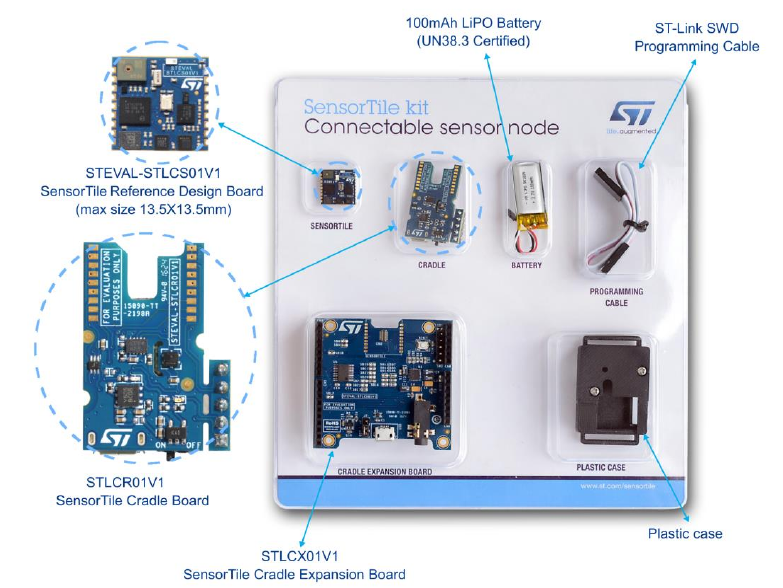
\includegraphics[scale=0.6]{sensortilekit}
\caption{SensorTile Development Kit}
\label{fig:sensortilekit}
\end{center} \end{figure}

\newpage

Figure \ref{fig:sensortile} shows position of main components of the SensorTile board, and Table \ref{table:sensortile} lists their description. \cite{stkitmanual}

\begin{figure}[H] \begin{center}
% \begin{wrapfigure}{l}{0.5\textwidth}
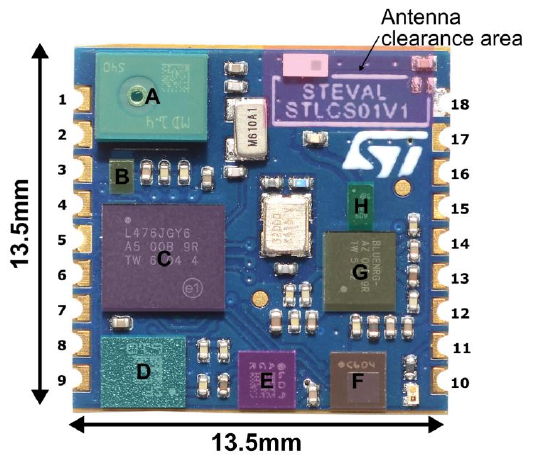
\includegraphics[scale=0.5]{sensortile}
\caption{SensorTile Main Components}
\label{fig:sensortile}
% \end{wrapfigure}
\end{center} \end{figure}

\begin{table}[H]
\centering
\begin{tabular}{@{}|c|l|p{0.55\linewidth}|@{}}
\hline
\toprule
{\bf Reference} & {\bf Device} & {\bf Description} \\ \hline
\midrule
A & MP34DT04      & MEMS audio sensor digital microphone \\ \hline
B & LD39115J18R   & 150 mA low quiescent current low noise LDO 1.8 V \\ \hline
C & STM32L476 MCU & ARM Cortex-M4 32-bit microcontroller \\ \hline
D & LSM6DSM       & iNEMO inertial module: low-power 3D accelerometer and 3D gyroscope \\ \hline
E & LSM303AGR     & Ultra-compact high-performance eCompass module: ultra-low power 3D accelerometer and 3D magnetometer \\ \hline
F & LPS22HB       & MEMS nano pressure sensor: 260-1260 hPa absolute digital output barometer \\ \hline
G & BlueNRG-MS    & Bluetooth low energy network processor \\ \hline
H & BALF-NRG01D3  & 50 Ω balun with integrated harmonic filter \\ \hline
\bottomrule
\end{tabular}
\caption{SensorTile Main Components}
\label{table:sensortile}
\end{table}

\newpage

By default, the SensorTile comes loaded

\newpage
\section{Android App}
\lipsum[1]

\newpage
\section{Analysis \& Results}
\lipsum[1]


% Conclusion & Future Work
\chapter{Conclusion}

\lipsum[2]


\bibliographystyle{plain}
\bibliography{biblio}

% \appendix
% \chapter{CHAPTER NAME}

\section{SECTION NAME}
\lipsum[1]

\section{SECTION NAME}
\lipsum[2]

\end{document}

